\documentclass{article}
\usepackage{graphicx} % Required for inserting images
\usepackage{float}
\title{Assignemnt 1}
\date{October 8, 2023}
\author{
  Ravi Raghavan\\
  \texttt{rr1133}
  \and
  Michelle Han\\
  \texttt{mmh255}
}

\begin{document}
\maketitle
\section{Generate, visualize and store 2D polygonal scenes}

\subsection{Example Maps}
The density of the maps was controlled by the amount of polygons in relation to the radii. Maps with greater radii (Fig. 1) required less polygons to fill the space compared to maps with smaller radii (Fig. 2). The shape of the polygons was controlled by the number of vertices. Maps with higher number of vertices resulted in polygons that were more round in appearance (Fig. 3 and 4). Maps with a lower amount of vertices appeared more sharp (Fig. 1 and 2). The four maps generated using \textit{constructScene} and their corresponding parameters:
\subsubsection{Big and Dense Polygons (see Fig. 1)}
Number of Polygons: 10
\\Minimum Number of Vertices: 4\space\space\space\space\space\space Maximum Number of Vertices: 6
\\Minimum Radius: 0.3\space\space\space\space\space\space\space\space\space\space\space \space\space\space\space\space\space \space\space\space Maximum Radius: 0.4
\subsubsection{Small and Dense Polygons (see Fig. 2)}
Number of Polygons: 30 
\\Minimum Number of Vertices: 4 \space\space\space\space\space\space Maximum Number of Vertices: 6
\\Minimum Radius: 0.1 \space\space\space\space\space\space\space\space\space\space\space \space\space\space\space\space\space \space\space\space Maximum Radius: 0.2
\subsubsection{Small and Sparse Polygons (see Fig. 3)}
Number of Polygons: 5
\\Minimum Number of Vertices: 15 \space\space\space\space\space\space Maximum Number of Vertices: 20
\\Minimum Radius: 0.05 \space\space\space\space\space\space\space\space\space\space\space \space\space\space\space\space\space \space\space\space Maximum Radius: 0.1
\subsubsection{Big and Sparse Polygons (see Fig. 4)}
Number of Polygons: 3
\\Minimum Number of Vertices: 5 \space\space\space\space\space\space Maximum Number of Vertices: 15 
\\Minimum Radius: 0.4 \space\space\space\space\space\space\space\space\space\space\space \space\space\space\space\space\space \space\space\space Maximum Radius: 0.6
\begin{figure}[htbp]
  \centering
  \begin{minipage}{0.45\textwidth}
    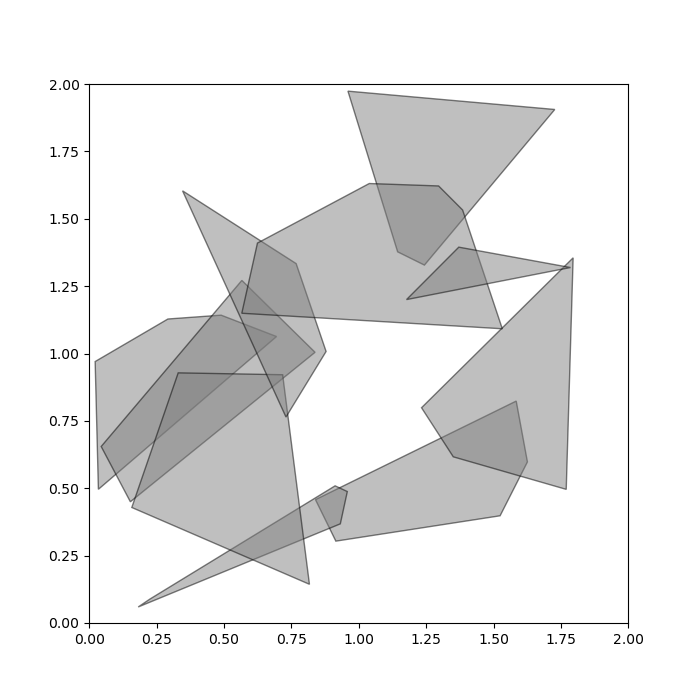
\includegraphics[width=\linewidth]{part1_big_dense.png}
    \caption{Big and dense polygons}
  \end{minipage}\hfill
  \begin{minipage}{0.45\textwidth}
    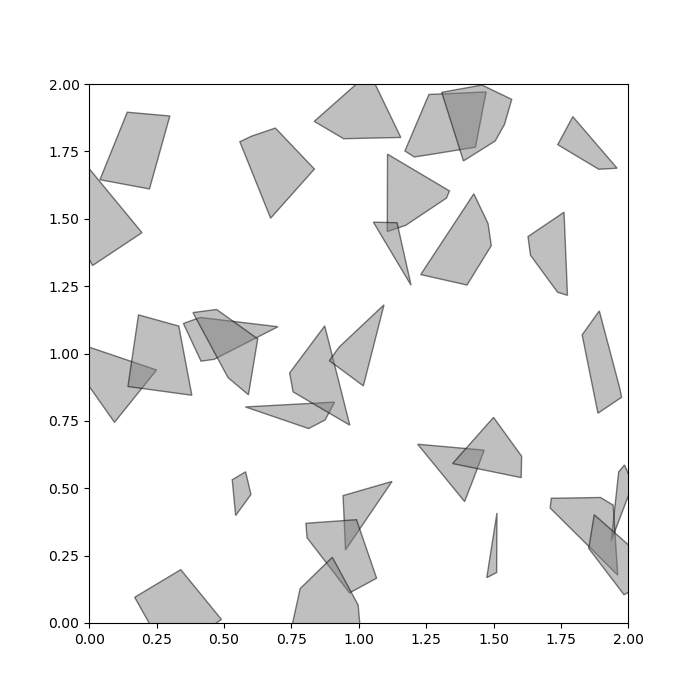
\includegraphics[width=\linewidth]{part1_small_dense.png}
    \caption{Small and dense polygons}
  \end{minipage}
  \begin{minipage}{0.45\textwidth}
    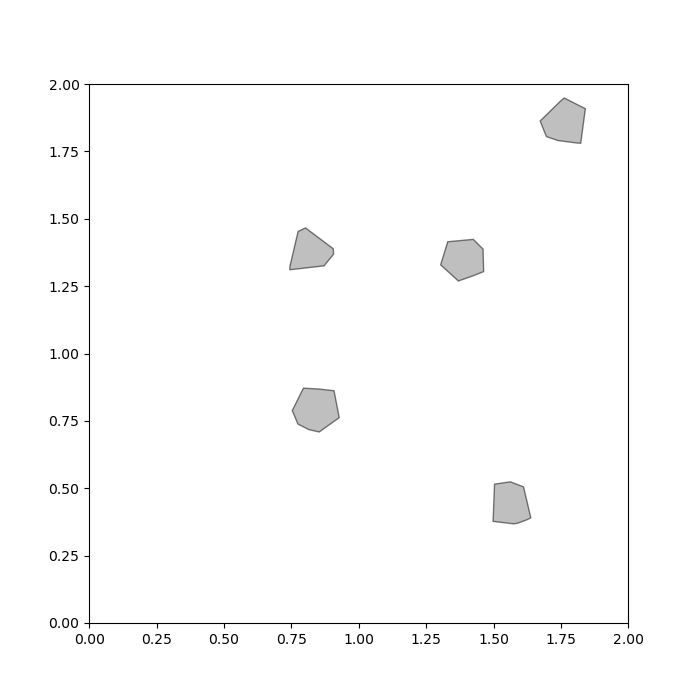
\includegraphics[width=\linewidth]{part1_small_sparse.png}
    \caption{Small and sparse polygons}
  \end{minipage}\hfill
  \begin{minipage}{0.45\textwidth}
    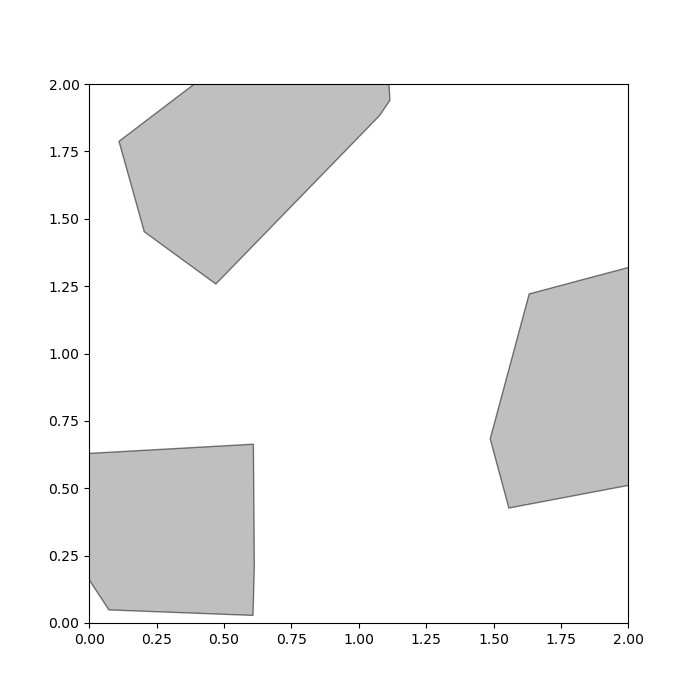
\includegraphics[width=\linewidth]{part1_sparse_big.png}
    \caption{Big and sparse polygons}
  \end{minipage}
\end{figure}

\subsection{Convex Polygon Letters}
\begin{figure}[H]
  \centering
  \begin{minipage}{0.45\textwidth}
    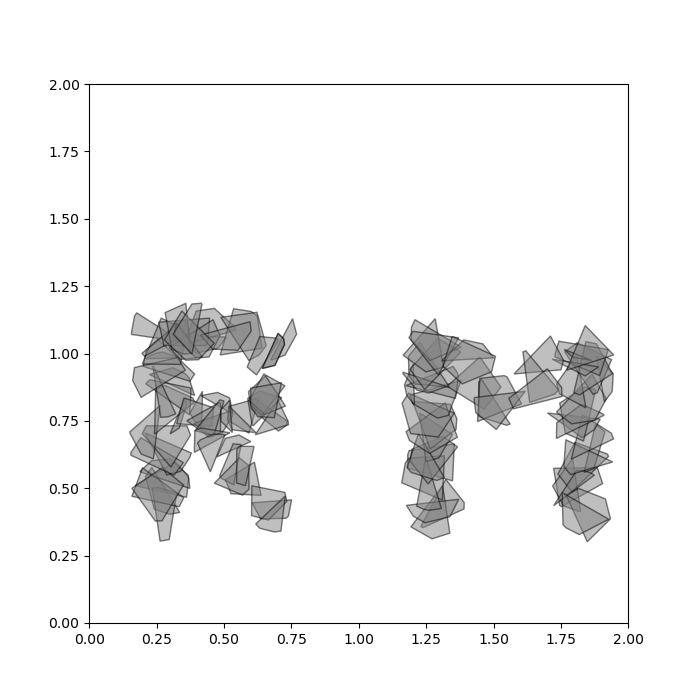
\includegraphics[width=\linewidth]{part1_letters.png}
    \caption{R and M generated using convex polygons}
  \end{minipage}\hfill
\end{figure}
\subsection{Convex Polygon Strategy}
In order to generate convex polygons, the strategy outlined in the write up was followed.
\subsubsection{Polygon Rotation}
A randomly sampled vertex (\textit{xcenter , ycenter}) was created inside the 2mx2m map. Using this vertex as the center, the minimum radius \textit{rmin} was used to generate a circle of radius \textit{rmin}. An angle, $\theta$, is sampled from [0°,360°]. A vertex is calculated by: 
    \[x = xcenter + r*cos(\theta)\]
    \[y = ycenter + r*sin(\theta)\]
 The expressions determine where the vertice falls on the circle. This is repeated N times to get N vertices from [\textit{nmin, nmax}]. The placement of the vertices along the circumference of a circle of radius \textit{rmin} allows for the polygon to be rotated.
\subsubsection{Extrude Vertices}
To extrude a vertex, a radius \textit{r} is sampled from [0, maximum vertices - minimum vertices]. The range [0, maximum vertices - minimum vertices] allows for a vertex to lie outside of the polygon's minimum radius. It allows for the circle that the new vertex lies on to be equal to or greater than radius \textit{rmin}. The new position of the vertex is calculated by: 
    \[new x = x + r*cos(\theta)\]
    \[new y = y + r*sin(\theta)\]
This process is repeated for all the vertices in the polygon. 
\subsubsection{Convexity of Polygons}
To determine the convexity of a generated polygon, the \textit{ConvexHull} function was used. The \textit{makeConvex} function takes a polygon and applies \textit{ConvexHull} to it. The result is the indices of vertices that form a convex polygon in counterclockwise order. This is stored in \textit{hull}. The indices in \textit{hull} are used to extract the vertices of the polygon that form a convex polygon into \textit{vertices}. Another vertex, the first one, is appended to \textit{vertices} so that the polygon is closed. \textit{convexPolygons} is ordered in counterclockwise order. If the given polygon is already convex, then convexPolygons will receive the same amount of vertices as the original polygon. 

\section{2D collision checking for convex polygons}
\section{Collision-free Navigation for a 2D rigid body}
\section{Collision-free Movement of a Planar Arm}
\subsection{Controlling Planar Arm}
To control the first joint, the up key increments by $\pi$/30 and the down key decrements by $\pi$/30. To control the second joint, the right key increments by $\pi$/30 and the left key decrements by $\pi$/30.
\subsection{Visualization of Scenes}

\begin{figure}[htbp]
  \centering
  \begin{minipage}{0.45\textwidth}
    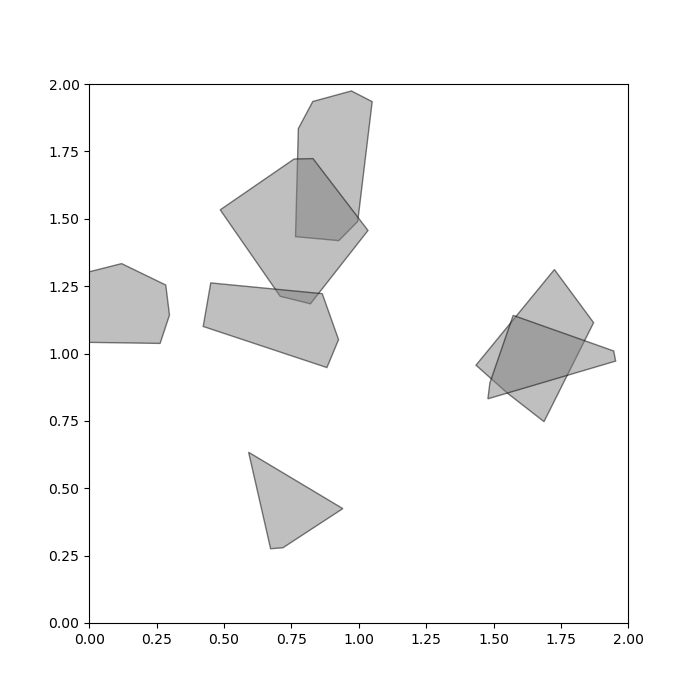
\includegraphics[width=\linewidth]{part4_without_arm.png}
  \end{minipage}\hfill
  \begin{minipage}{0.45\textwidth}
    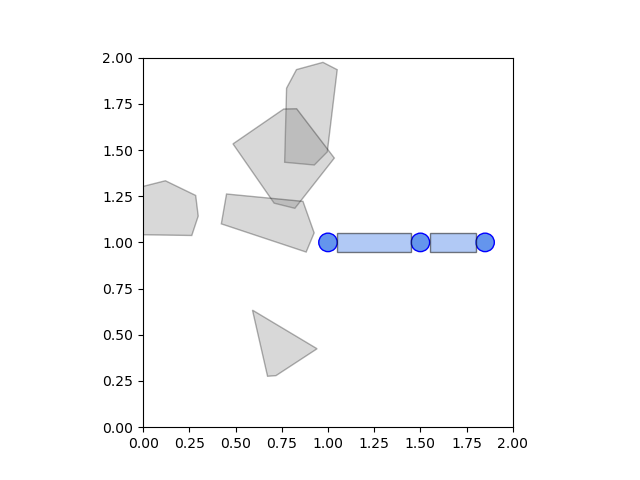
\includegraphics[width=\linewidth]{part4_with_arm.png}
  \end{minipage}
    \caption{Polygons that collide with arm at start are removed}
\end{figure}

\subsection{Collision-Free Configuration Space}
\begin{figure}[htbp]
  \centering
  \begin{minipage}{0.45\textwidth}
    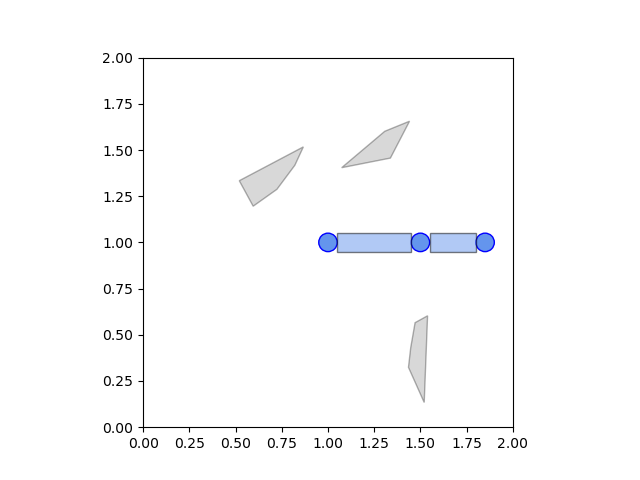
\includegraphics[width=\linewidth]{part4_arm_free.png}
    \caption{Arm collision-free}
  \end{minipage}\hfill
\end{figure}


\end{document}
